\section{Procedimento Experimental}

\subsection{Local, Arquitetura e Lógica de Montagem}

A montagem e a verificação experimental foram realizadas em \textit{protoboard} de $830$ pontos nas bancadas do Laboratório de Redes e Eletrônica da FACOM/UFMS. A montagem seguiu o encadeamento dos estágios de conversão de energia, o que permitiu testar cada bloco antes de integrar a carga final. O diagrama completo do circuito é apresentado na Figura~\ref{fig:esquematico}, e os pontos de medição dos experimentos estão indicados por E1 a E6. O regulador LM7812 foi utilizado sem dissipador de calor.

\begin{figure*}[t]
\centering
\resizebox{0.96\textwidth}{!}{%
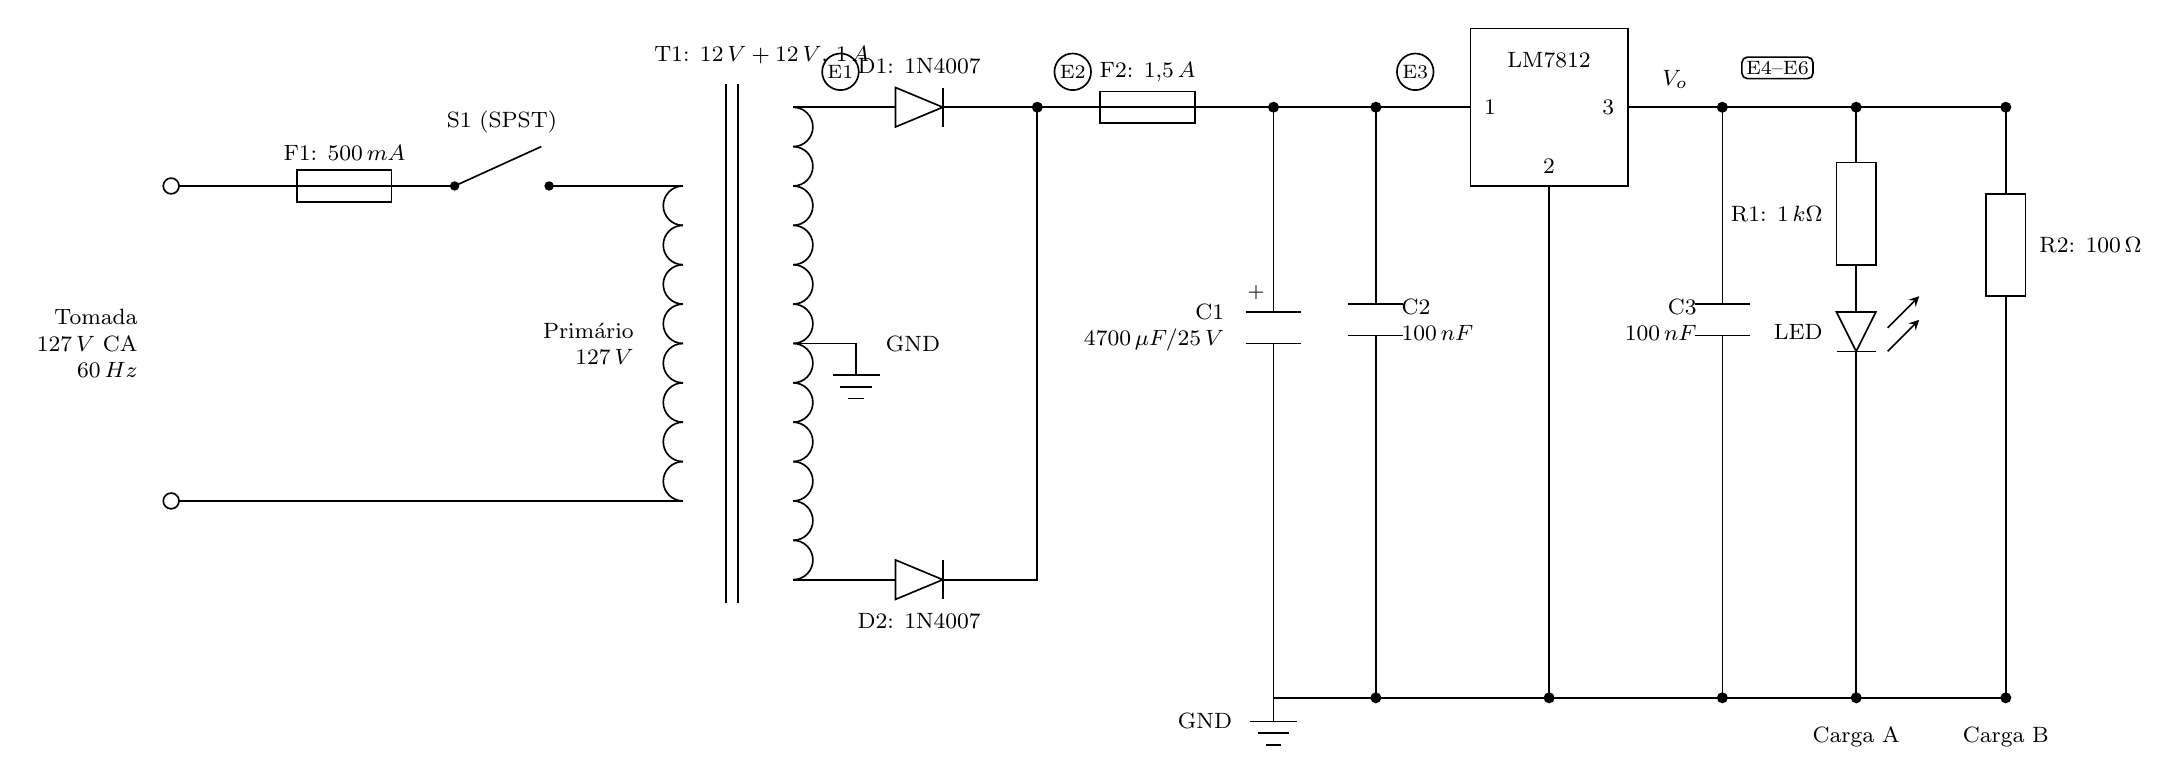
\begin{tikzpicture}[line width=0.6pt,>=stealth,font=\footnotesize]
% --- Tomada, F1 e chave S1 (primario)
\draw (0,5) circle (0.1);
\draw (0,1) circle (0.1);
\node[anchor=east,align=right] at (-0.3,3) {Tomada\\$127\,\text{V}$ CA\\$60\,\text{Hz}$};
\draw (0.1,5)--(1.6,5);
\draw (0.1,1)--(6.5,1);
\draw (1.6,4.8) rectangle (2.8,5.2);
\draw (1.6,5)--(2.8,5);
\node[above] at (2.2,5.2) {F1: $500\,\text{mA}$};
\draw (2.8,5)--(3.6,5);
\fill (3.6,5) circle (0.06);
\fill (4.8,5) circle (0.06);
\draw (3.6,5)--(4.7,5.5);
\draw (4.8,5)--(6.5,5);
\node[above] at (4.2,5.55) {S1 (SPST)};
% --- Transformador T1 (primario, nucleo, secundario com derivacao central)
\foreach \i in {0,...,7} {\draw (6.5,{5-\i*0.5}) arc (90:270:0.25);}
\node[anchor=east,align=right] at (6.0,3) {Primário\\$127\,\text{V}$};
\draw (7.05,-0.3)--(7.05,6.3);
\draw (7.2,-0.3)--(7.2,6.3);
\foreach \i in {0,...,11} {\draw (7.9,{6-\i*0.5}) arc (90:-90:0.25);}
\node[above,align=center] at (7.5,6.4) {T1: $12\,\text{V}+12\,\text{V}$, $1\,\text{A}$};
% derivacao central (GND)
\draw (7.9,3)--(8.7,3);
\draw (8.7,3)--(8.7,2.6);
\draw (8.4,2.6)--(9.0,2.6);
\draw (8.5,2.45)--(8.9,2.45);
\draw (8.6,2.3)--(8.8,2.3);
\node[right] at (8.95,3) {GND};
% --- Diodos D1 e D2
\draw (7.9,6)--(9.2,6);
\draw[fill=white] (9.2,6.25)--(9.2,5.75)--(9.8,6)--cycle;
\draw (9.8,6.25)--(9.8,5.75);
\draw (9.8,6)--(11,6);
\node[above] at (9.5,6.3) {D1: 1N4007};
\draw (7.9,0)--(9.2,0);
\draw[fill=white] (9.2,0.25)--(9.2,-0.25)--(9.8,0)--cycle;
\draw (9.8,0.25)--(9.8,-0.25);
\draw (9.8,0)--(11,0)--(11,6);
\node[below] at (9.5,-0.3) {D2: 1N4007};
\fill (11,6) circle (0.07);
% --- Fusivel F2, capacitor C1 e trilho nao regulado
\draw (11,6)--(11.8,6);
\draw (11.8,5.8) rectangle (13,6.2);
\draw (11.8,6)--(13,6);
\node[above] at (12.4,6.2) {F2: $1{,}5\,\text{A}$};
\draw (13,6)--(16.5,6);
\fill (14,6) circle (0.07);
\draw (14,6)--(14,3.4);
\draw (13.65,3.4)--(14.35,3.4);
\draw (13.65,3.0)--(14.35,3.0);
\draw (14,3.0)--(14,-1.5);
\node at (13.78,3.65) {\scriptsize $+$};
\node[left,align=right] at (13.5,3.2) {C1\\$4700\,\mu\text{F}/25\,\text{V}$};
% --- Capacitor C2 (entrada do regulador)
\fill (15.3,6) circle (0.07);
\draw (15.3,6)--(15.3,3.5);
\draw (14.95,3.5)--(15.65,3.5);
\draw (14.95,3.1)--(15.65,3.1);
\draw (15.3,3.1)--(15.3,-1.5);
\fill (15.3,-1.5) circle (0.07);
\node[right,align=left] at (15.5,3.3) {C2\\$100\,\text{nF}$};
% --- Regulador LM7812
\draw (16.5,5) rectangle (18.5,7);
\node at (17.5,6.6) {LM7812};
\node at (16.75,6.0) {1};
\node at (18.25,6.0) {3};
\node at (17.5,5.25) {2};
\draw (17.5,5)--(17.5,-1.5);
\fill (17.5,-1.5) circle (0.07);
% --- Saida, capacitor C3 e cargas
\draw (18.5,6)--(23.3,6);
\fill (19.7,6) circle (0.07);
\draw (19.7,6)--(19.7,3.5);
\draw (19.35,3.5)--(20.05,3.5);
\draw (19.35,3.1)--(20.05,3.1);
\draw (19.7,3.1)--(19.7,-1.5);
\fill (19.7,-1.5) circle (0.07);
\node[left,align=right] at (19.5,3.3) {C3\\$100\,\text{nF}$};
\node at (19.1,6.35) {$V_o$};
% carga A: R1 + LED
\fill (21.4,6) circle (0.07);
\draw (21.4,6)--(21.4,5.3);
\draw (21.15,4.0) rectangle (21.65,5.3);
\draw (21.4,4.0)--(21.4,3.4);
\draw[fill=white] (21.15,3.4)--(21.65,3.4)--(21.4,2.9)--cycle;
\draw (21.15,2.9)--(21.65,2.9);
\draw (21.4,2.9)--(21.4,-1.5);
\fill (21.4,-1.5) circle (0.07);
\draw[->] (21.8,3.2)--(22.2,3.6);
\draw[->] (21.8,2.9)--(22.2,3.3);
\node[left] at (21.1,4.65) {R1: $1\,\text{k}\Omega$};
\node[left] at (21.1,3.15) {LED};
\node at (21.4,-2.0) {Carga A};
% carga B: R2
\fill (23.3,6) circle (0.07);
\draw (23.3,6)--(23.3,4.9);
\draw (23.05,3.6) rectangle (23.55,4.9);
\draw (23.3,3.6)--(23.3,-1.5);
\fill (23.3,-1.5) circle (0.07);
\node[right] at (23.6,4.25) {R2: $100\,\Omega$};
\node at (23.3,-2.0) {Carga B};
% --- Trilho de GND
\draw (14,-1.5)--(23.3,-1.5);
\draw (14,-1.5)--(14,-1.8);
\draw (13.7,-1.8)--(14.3,-1.8);
\draw (13.8,-1.95)--(14.2,-1.95);
\draw (13.9,-2.1)--(14.1,-2.1);
\node[left] at (13.6,-1.8) {GND};
% --- Marcadores de medicao
\node[draw,circle,inner sep=1pt,font=\scriptsize] at (8.5,6.45) {E1};
\node[draw,circle,inner sep=1pt,font=\scriptsize] at (11.45,6.45) {E2};
\node[draw,circle,inner sep=1pt,font=\scriptsize] at (15.8,6.45) {E3};
\node[draw,rounded corners=2pt,inner sep=1.5pt,font=\scriptsize] at (20.4,6.5) {E4--E6};
\end{tikzpicture}}
\caption{Diagrama esquemático da fonte de $12\,\text{V}$: tomada de $127\,\text{V}$, fusível F1 ($500\,\text{mA}$), chave S1, transformador T1 com derivação central (GND), diodos D1 e D2 (1N4007), fusível F2 ($1{,}5\,\text{A}$), capacitor C1 ($4700\,\mu\text{F}/25\,\text{V}$), regulador LM7812 (pinos 1, 2 e 3), capacitores C2 e C3 ($100\,\text{nF}$) e as cargas de ensaio (R1 + LED e R2). Em E2, o capacitor C1 foi removido e um resistor de $1\,\text{k}\Omega$ foi conectado ao GND na etapa sem filtro.}
\label{fig:esquematico}
\end{figure*}

\begin{enumerate}
    \item \textbf{Entrada AC e proteção primária:} O plugue conectado à rede elétrica de $127\,\text{V}$ passa por um porta-fusível volante com fusível de $500\,\text{mA}$ e segue para uma chave gangorra liga/desliga (SPST), que alimenta o enrolamento primário do transformador ($12\,\text{V}+12\,\text{V}$, $1\,\text{A}$).
    \item \textbf{Secundário e retificação:} O fio preto da derivação central do secundário foi ligado ao barramento de referência (GND) da \textit{protoboard}. Os dois fios vermelhos das extremidades do secundário foram conectados aos anodos de dois diodos 1N4007, cujos catodos foram interligados em um mesmo nó.
    \item \textbf{Proteção secundária e filtragem:} Do nó comum dos catodos, um fio conduz o sinal retificado por um segundo porta-fusível volante, com o fusível de $1{,}5\,\text{A}$, até o barramento positivo da \textit{protoboard} (nó de tensão não regulada). Sobre esse nó ligam-se em paralelo o capacitor eletrolítico de $4700\,\mu\text{F} / 25\,\text{V}$ (terminal positivo na linha retificada e negativo no GND), o primeiro capacitor de $100\,\text{nF}$ e o pino~1 (entrada) do LM7812.
    \item \textbf{Regulação e saída:} O pino~2 (GND) do LM7812 conecta-se ao barramento de referência. O pino~3 (saída regulada de $12\,\text{V}$) liga-se ao segundo capacitor de $100\,\text{nF}$, em paralelo com o GND, e aos pontos de conexão das cargas de ensaio (LED em série com resistor de $1\,\text{k}\Omega$, e resistor de $100\,\Omega$).
\end{enumerate}

\textbf{Segurança.} O primário do transformador é alimentado pela rede por meio do plugue, de um fusível e de uma chave, e o transformador permaneceu fora da \textit{protoboard}, de modo que apenas o secundário de baixa tensão foi levado à \textit{protoboard}. Recomenda-se desligar a montagem da tomada antes de remover ou inserir componentes, como foi feito na troca do capacitor e do resistor no Experimento~2, e manter isoladas as conexões do lado da rede.

\subsection{Materiais Utilizados e Custos}

Para os ensaios foram empregados um multímetro digital Victor~88B (Skill-Tec) e um osciloscópio digital Gratten GA1102CAL ($100\,\text{MHz}$, $1\,\text{GSa/s}$). A Tabela~\ref{tab:bom} relaciona os componentes e acessórios adquiridos e utilizados na construção da fonte e nos testes.

\begin{table}[H]
\caption{Lista de componentes utilizados na montagem e custos em reais.}
\label{tab:bom}
\centering
\scriptsize
\setlength{\tabcolsep}{3pt}
\begin{tabular}{cp{6.5cm}}
\hline
Qtd. & Componente / Especificação \\
\hline
1 & Transformador $127/220\,\text{V} \to 12+12\,\text{V}$ ($1\,\text{A}$) \\
1 & Regulador de tensão LM7812 ($12\,\text{V}$, TO-220) \\
1 & Capacitor eletrolítico $4700\,\mu\text{F} / 25\,\text{V}$ \\
2 & Capacitores $100\,\text{nF}$ (104) \\
2 & Diodos retificadores 1N4007 \\
2 & Porta-fusíveis \textit{inline} + fusíveis ($500\,\text{mA}$ e $1{,}5\,\text{A}$); tipo e tensão nominal não especificados pelo vendedor \\
1 & Chave gangorra liga/desliga (SPST) \\
1 & Plugue macho 2P padrão NBR 14136 ($10\,\text{A}$) \\
1 & \textit{Protoboard} $830$ pontos \\
1 & Kit LED $5\,\text{mm}$, resistores ($1\,\text{k}\Omega$; $100\,\Omega$) e fios \\
\hline
\textbf{Total:} & \textbf{R\$ 133} \\
\hline
\end{tabular}
\end{table}

\subsection{Metodologia dos Ensaios Experimentais}

A caracterização da fonte foi conduzida em seis experimentos sequenciais, da saída alternada do transformador até a regulação de carga e a corrente na saída final. Nas capturas do osciloscópio, o fator de atenuação configurado no canal e a posição da chave da ponta nem sempre coincidiram; por isso, os resultados são apresentados como valor exibido, fator aplicado e valor real (Seção~\ref{sec:analise}).

\begin{enumerate}
    \item \textbf{Experimento 1 --- Saída do transformador (pré-retificação):} Sem carga na saída de $12\,\text{V}$, a referência (garra) foi posicionada no fio preto central (GND) e a ponta de medição em um dos terminais vermelhos do secundário, antes dos diodos. O osciloscópio foi utilizado em acoplamento DC. O multímetro permaneceu na escala de $20\,\text{V}$ DC, e não em V$\sim$ (tensão alternada); trata-se de um erro de procedimento, e a leitura obtida não é resultado válido do ensaio.
    \item \textbf{Experimento 2 --- Onda pós-diodos (sem e com filtro capacitivo):} Com a montagem desligada da tomada, o capacitor eletrolítico de $4700\,\mu\text{F}$ foi removido e um resistor de $1\,\text{k}\Omega$ foi inserido entre o nó pós-fusível e o GND. A forma de onda foi registrada no osciloscópio em acoplamento DC. Em seguida, com a montagem novamente desligada, o resistor foi retirado, o capacitor foi reinstalado e a captura foi repetida.
    \item \textbf{Experimento 3 --- Filtro e \textit{ripple} antes do LM7812 (pino 1):} A tensão DC no pino~1 foi medida com o multímetro (escala $20\,\text{V}$ DC). Em seguida, o osciloscópio em acoplamento AC, com $2{,}00\,\text{mV/div}$, $5{,}00\,\text{ms/div}$, limite de banda (B) e filtro (F) ativos, registrou a ondulação em duas condições: saída de $12\,\text{V}$ em aberto e, depois, com LED em série com resistor de $1\,\text{k}\Omega$ entre o pino~3 e o GND. A posição da chave $1\times$/$10\times$ da ponta não foi registrada.
    \item \textbf{Experimento 4 --- Saída regulada de $12\,\text{V}$ (pino 3):} Com o LED e o resistor de $1\,\text{k}\Omega$ conectados na saída, mediram-se a tensão DC no pino~3 com o multímetro ($20\,\text{V}$ DC) e o sinal residual com o osciloscópio em acoplamento AC ($2{,}00\,\text{mV/div}$, $5{,}00\,\text{ms/div}$, B e F ativos). A posição da chave da ponta também não foi registrada.
    \item \textbf{Experimento 5 --- Regulação de carga:} Com o multímetro na escala de $20\,\text{V}$ DC entre o pino~3 e o GND, compararam-se as leituras sem carga (LED desconectado) e com a carga de ensaio (LED + resistor de $1\,\text{k}\Omega$).
    \item \textbf{Experimento 6 --- Corrente com carga de $100\,\Omega$:} Um resistor de $100\,\Omega$ foi conectado ao GND e o multímetro foi inserido em série entre o pino~3 do LM7812 e o outro terminal do resistor. A ponta vermelha foi conectada ao borne de $20\,\text{A}$ e a ponta preta ao borne COM, e a corrente indicada foi $0{,}12\,\text{A}$. Na fotografia, a posição do seletor não coincide com o borne utilizado, e a resolução da indicação é de $0{,}01\,\text{A}$.
\end{enumerate}
